\documentclass[a4paper,10pt]{article}
\usepackage[a4paper, left=3cm,right=2.5cm]{geometry}

\usepackage[spanish]{babel}
\selectlanguage{spanish}
\usepackage[utf8]{inputenc}
\usepackage[pdftex]{graphicx}

% Utilizado para recuadrar expresiones
\usepackage{amsmath}
% Recuadros con mayor separación
\setlength{\fboxsep}{6pt}

\def \anio {a\tilde{n}o}

\begin{document}

\paragraph{Ejercicio 1} A continuación se presenta la red, con el camino crítico resaltado en trazo grueso; esta comprende las actividades B, C, D, E y J. La duración del proyecto es de 23 semanas.

    \begin{center}
	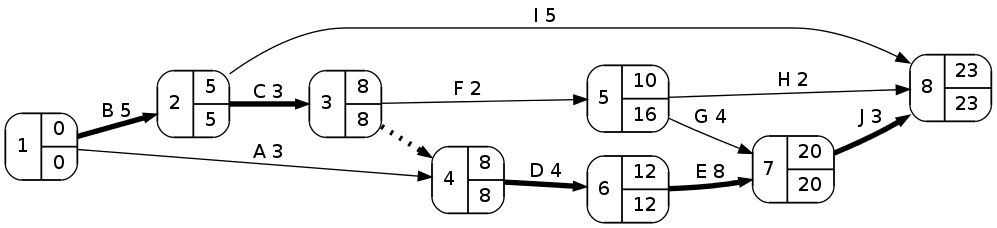
\includegraphics[scale=0.55,keepaspectratio=true]{img/ej1-red.png} 
	\end{center}
  
\paragraph{Ejercicio 3}
  Para encontrar el camino crítico, se obtiene el grafo de tareas representado por la matriz de precedencia y, sobre el mismo, se ejecuta el algoritmo de búsqueda de camino crítico.

  \begin{center}
    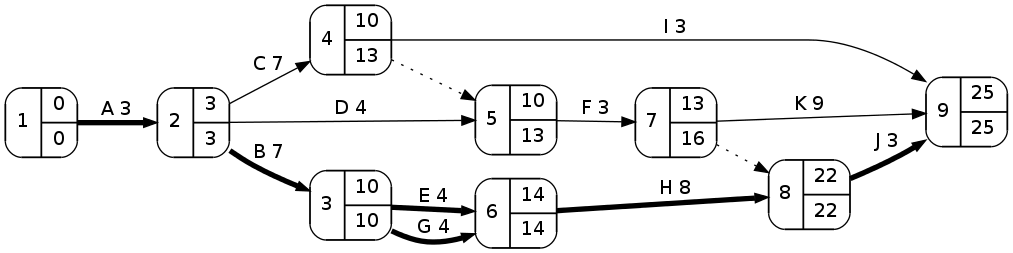
\includegraphics[scale=0.4,keepaspectratio=true]{img/ej3-0.png} 
  \end{center}

  El este gráfico puede verse el proyecto inicial, con los caminos críticos resaltados en trazo más grueso y las tareas ficticias en líneas punteadas.

  Los caminos críticos son: A-B-E-H-J y A-B-G-H-J.

  La duración del proyecto es de 25 semanas. Y, su costo, es de \$$14600$ (se obtiene sumando el costo de cada tarea, consistente en el producto de su duración por el costo semanal de la misma).

  \subparagraph{Reducción de la duración del proyecto}

  Para poder decidir el orden en que se reducirán las tareas, se calcula el costo de reducción semanal de cada una. Éste se obtiene como el cociente entre el costo de reducción total ($\Delta \$$ o costo crash menos costo) y su máxima reducción posible ($\Delta d$ o diferencia entre tiempo normal y tiempo mínimo).

   \begin{center}
   \begin{tabular}{|| c | c | c | c ||}
   \hline 
      Tarea & $\Delta d$ & $\Delta \$$ & $\Delta \$ / \Delta d$ \\ \hline \hline
      A & 1 & 100 & 100 \\ \hline
      B & 1 & 140 & 140 \\ \hline 
      C & 2 & 400 & 200 \\ \hline
      D & 2 & 500 & 250 \\ \hline
      E & 2 & 400 & 200 \\ \hline
      F & 2 & 600 & 300 \\ \hline
      G & 3 & 900 & 300 \\ \hline
      H & 0 &  -  & -   \\ \hline
      I & 1 &1000 & 1000\\ \hline
      J & 0 &  -  & -   \\ \hline
      K & 3 & 300 & 100 \\ \hline
   \end{tabular}
   \end{center}

   Puede verse en la tabla que la tarea crítica con menor costo de reducción semanal es A. Sin embargo ésta puede reducirse a lo sumo en una semana. Por lo tanto, si conviene, deberá luego reducirse otra tarea.

  \subparagraph {Reducción en una semana de la tarea A}
  \begin{center}
    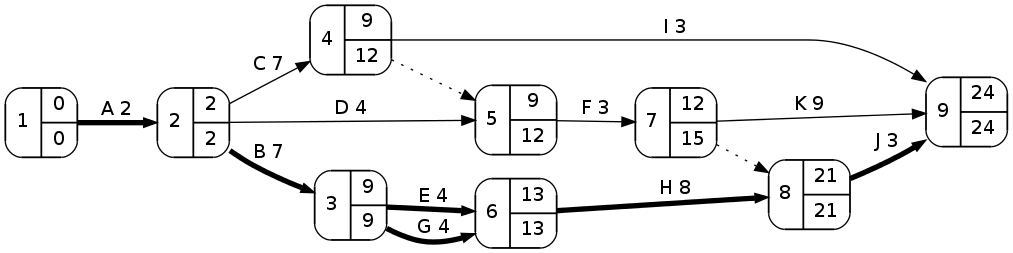
\includegraphics[scale=0.4,keepaspectratio=true]{img/ej3-1.png} 
  \end{center}

  Al haber reducido una tarea crítica en una semana, la nueva duración del proyecto es de 24 semanas. Y su nuevo costo, dado el beneficio otorgado por esta reducció, es de $\$14600 - \$150 + \$100 = \$14550$. Por lo tanto, conviene reducir el proyecto en una semana.


  Ahora, la tarea crítica con menor costo de reducción semanal es B.

  \subparagraph {Reducción en una semana de la tarea B}
  \begin{center}
    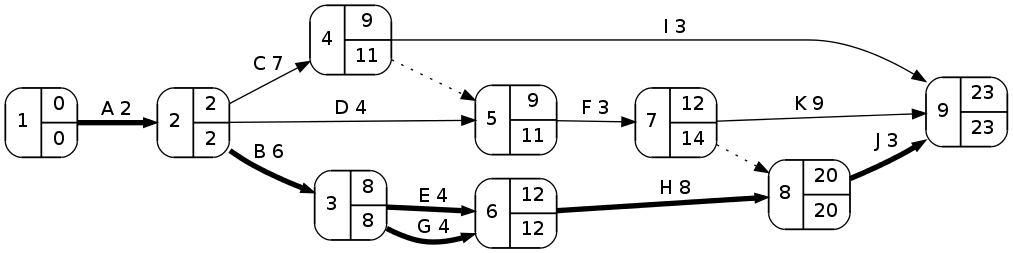
\includegraphics[scale=0.4,keepaspectratio=true]{img/ej3-2.png} 
  \end{center}

  Nuevamente bajó la duracción del proyecto, a un total de 23 semanas. Y su costo ahora es de $\$14550 - \$150 + \$140 = \$14540$. Entonces conviene aceptar la reducción de 25 a 23 semanas.

  \subparagraph {Reducción de la tercer semana}
  Ahora, la única reducción posible en tareas que formen parte de un camino crítico es en E y G. Dado que ambas no forman parte del mismo camino, deben reducirse en simultáneo.

  El costo de reducir en una semana E es de $\$200$, y el de G es de $\$300$, por lo que no conviene si el beneficio percibido es de $\$150$ en total ya que el nuevo costo llegaría a ser de $\$14540 + \$200 + \$300 - \$150 = \$14890$, siendo mayor que el original del proyecto.
\end{document}
